\documentclass[a4paper]{article}
\usepackage[utf8]{inputenc}
\usepackage{graphicx}
\usepackage{amsmath}
\usepackage[bottom=2.0cm,top=2.0cm,left=2.0cm,right=2.0cm]{geometry}
\usepackage[english]{babel}
\usepackage{indentfirst}
\usepackage{hyperref}  
\hypersetup{colorlinks,citecolor=black,filecolor=black,linkcolor=black,urlcolor=black}
\usepackage[nottoc]{tocbibind}
\usepackage{lipsum}
\usepackage{blindtext}
\usepackage{pdfpages}
\usepackage{epsfig} %% for loading postscript figures
\usepackage{listings}
\usepackage{hyperref}
\usepackage{amssymb}
\usepackage{setspace}
\usepackage{fancyhdr}

\pagestyle{fancy}
\fancyhf{}
\renewcommand{\headrulewidth}{0pt}

\rfoot{\thepage \hspace{1pt}}

\doublespace
\begin{document}
\title{Engineering Report}


\begin{titlepage}
	\begin{center}
		\begin{figure}[htb!]
			\begin{flushleft}
				
\includegraphics[width=3.9cm]{images/fau_logo.jpeg}
			\end{flushleft}
		\end{figure}
        \vspace{-2.5cm}
        \hspace{2.1cm}\Large{\textbf{Florida Atlantic University}}\\
        \hspace{2.1cm}\Large{College of Engineering}\\
        
        \vspace{200pt}
        
        \LARGE{\textbf{Project 1}}\\ 
        \Large{Application of the Direct Integration Method or of Discontinuity (Singularity) Functions to Statically Determinate Uniform or Stepped Beam Design}\\ 
        
        \vspace{100pt}
        
        \hfill Serial Number: 02 \\
        
        \vspace{30pt} 
        \hfill Name: Pedro Almeida\\
        \hfill Professor Name: Dr. Isaac Elishakoff\\
        \hfill TA Name: Abhishek Ratanpara\\
        \hfill Student Email: palmeida2016@fau.edu\\
        \hfill Telephone Number: +1 (561) 480-5483\\
        
        
        \vspace{\fill}
        \LARGE \bf{\today}
          
	\end{center}
\end{titlepage}


\includepdf[pages=-]{assignment/project1_probs.pdf}
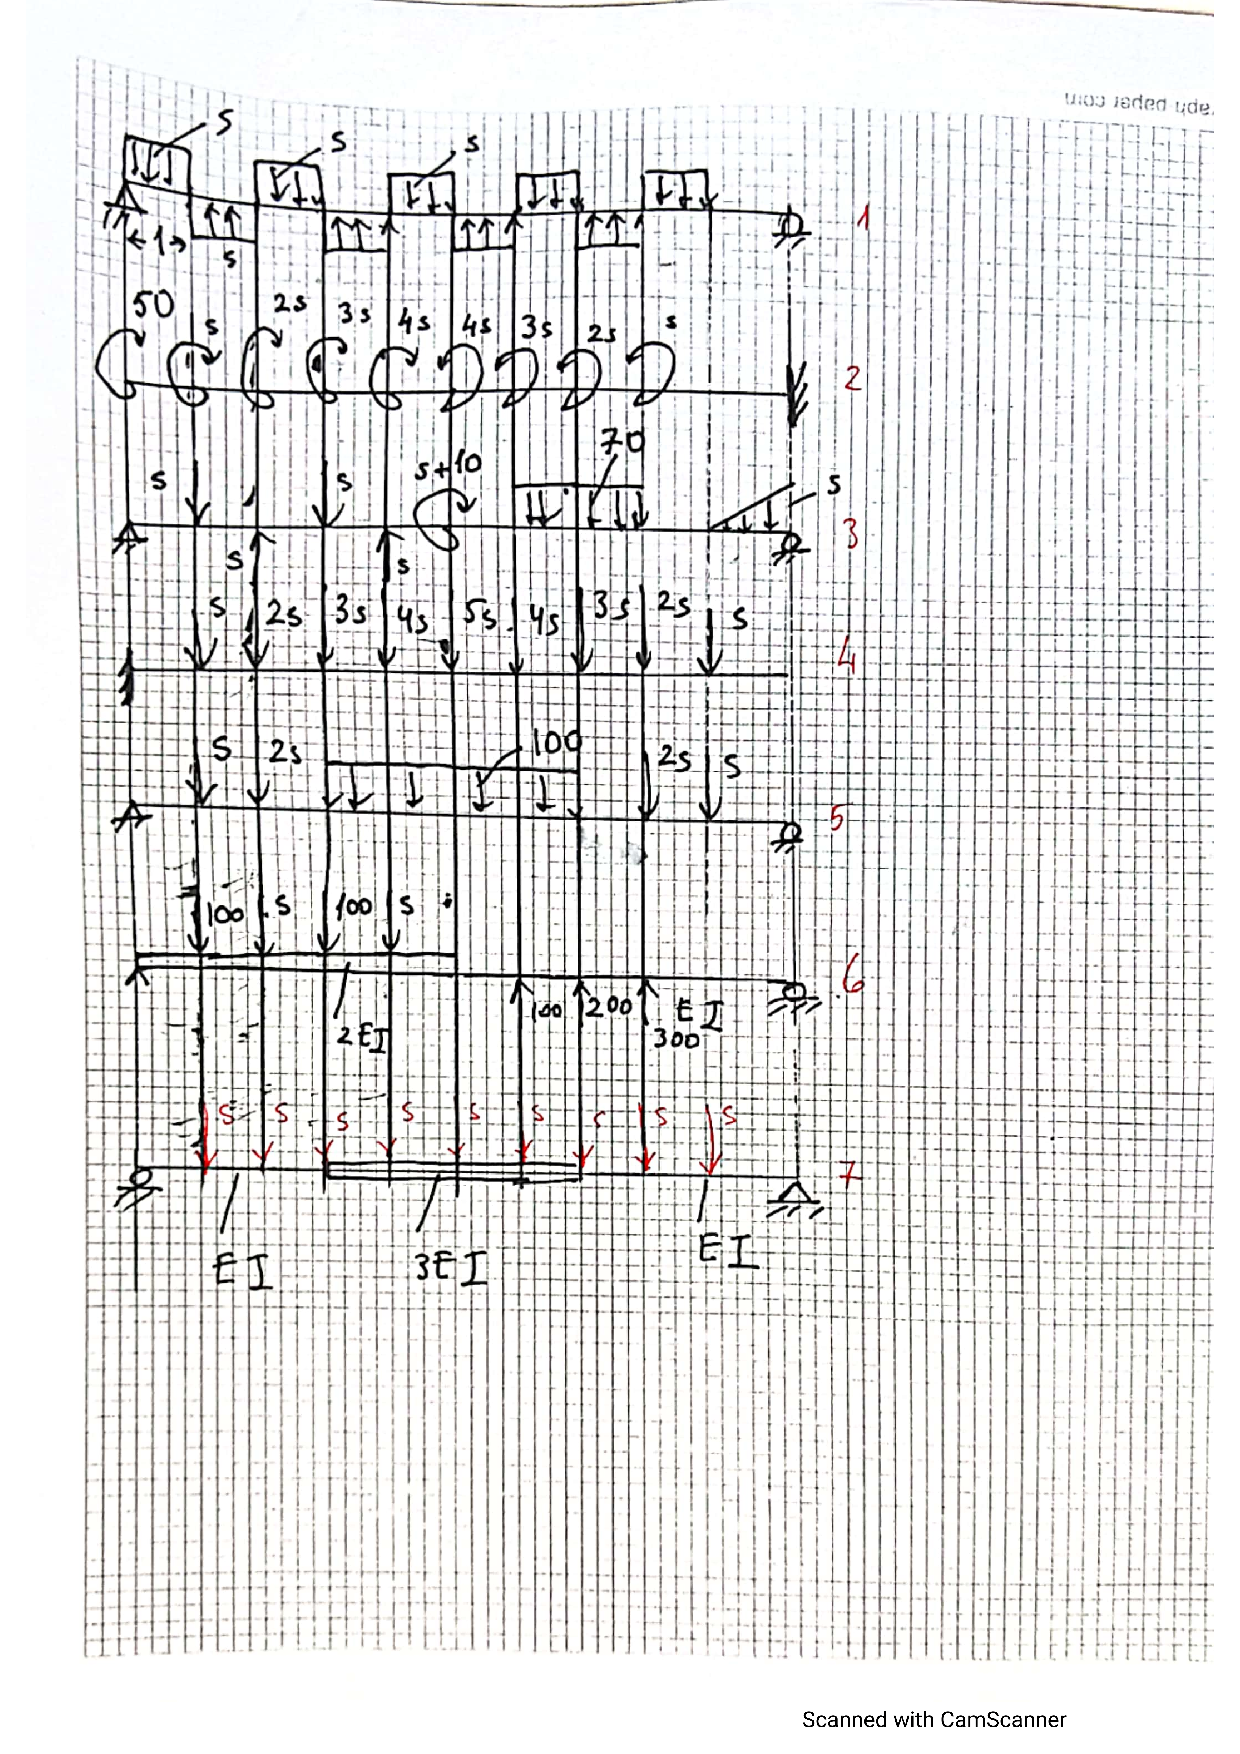
\includepdf[pages=-]{assignment/project1_dwg.pdf}

\large
\textit{The report will apply the Direct Integration Method of Singularity Functions to statically determine uniform or stepped beam designs to determine the load's effect on the beam's deflection. The resulting functions following the integration will be plotted using MATLAB software to produce simplified renderings of the beam's shape post loading.}

\tableofcontents

\section{Introduction} \label{Introduction}
One of the most important processes in designing beams is the structural analysis of the part under realistic loading conditions. A proper, realistic, theoretical model allows the engineer or designer to understand the expected stresses and deflections of a beam under expected loading conditions, thus removing the need to conduct experiments for each attempted revision. To properly construct the theoretical models, engineers often rely on extensive sets of equations.

The standard method to solve for beam deflection for beams with continuous cross sectional areas relies on partitions; the designer splits the beam into multiple subsections where loads are applied. The resulting cross sections are then each modeled separately. The singularity equations for beam deflection, by contrast, allow for the reduction of the multiple deflection equations into a single continuous equation. The method will be discussed thoroughly in the \nameref{Background Theory} section.

The report will comprise of the \nameref{Background Theory} section discussing the required equations and methods to solve the problems, the \nameref{Problems} section discussing each of the problems presented in the project, the \nameref{Solutions} section discussing the steps used to arrive to each solution, the \nameref{Results} containing the important plots for each of the problems given, and the \nameref{Conclusions} section to summarize findings and discuss improvements.

\section{Background Theory} \label{Background Theory}
To find the deflection equation for a statically determinate beam under loading, there are two principal ways to approach the problem, both of which lead to the same result. The first method, shown in Eq. \ref{form1}, uses the loading function $w(x)$ to reach the deflection. The form is especially useful for beams under non-linear loading functions. However, due to the required quadruple integration to reach $v(x)$, engineers commonly use a second form.

\begin{equation}
    EI \frac{\delta^4 v}{\delta x^4} = w(x)
\label{form1}
\end{equation}

The second form of the deflection equation can be given by Eq. \ref{form3}. The function utilizes the moment function $W(x)$ and a double integration to model the deflection, generating 2 constants of integration rather than 4. As such, if possible, the second form is preferred. With the form of integration determined, the engineering must then determine the moment function applied onto the beam as a function of the loads, which begins by statically solving the problem.

\begin{equation}
    EI \frac{\delta^2 v}{\delta x^2} = M(x)
\label{form3}
\end{equation}

The first step to find the static forces acting on a beam includes the decomposition of the applied and reaction forces onto a Free Body Diagram (FBD). To define the FBD, the report must first determine the type of supports acting on the beam. For a simply supported beam, the pin support creates a reaction $x$ and $y$ directions, while the roller support only creates a reaction in the $y$ direction. For a wall support, the beam must have a reaction in the $x$ and $y$ directions in addition to a moment reaction. Fig. \ref{FBD_example} shows an example of a FBD decomposition.

\begin{figure}[h]
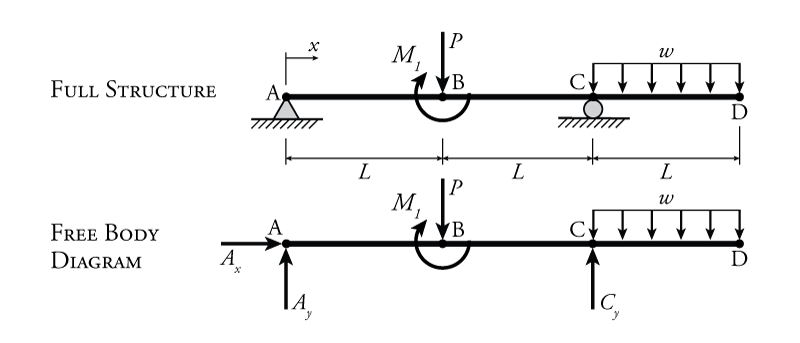
\includegraphics[width=\textwidth]{FBD/FBD_example.jpeg}
\caption{Example Free Body Diagram}
\label{FBD_example}
\end{figure}

With the FBD drawn, the report uses the set of equations shown in Eq. \ref{static_equations} to solve for the reaction forces. In most scenarios, the horizontal force $F_x$, and therefore the horizontal reaction, will be equal to zero, leaving 2 main equations to be used to solve for the vertical reactions at each of the supports. 

\begin{equation}
    \begin{split}
    &\uparrow \sum F_y = 0 \\
    &\rightarrow \sum F_x = 0 \\
    &\circlearrowleft \sum M_A = 0
    \end{split}
\label{static_equations}
\end{equation}

Once the support reactions have been found, the engineer proceeds by selecting Eq. \ref{form1} or Eq. \ref{form3} to apply. For the purposes of the example, Eq. \ref{form3} will be used. For that form, the report sets an $x$-$y$ coordinate system on the left side of the beam such that the $x$ axis extends along the beam and the $y$ axis extends perpendicular to the length of the beam. With the coordinate system established, the report constructs the Moment equation based on Eq. \ref{moment_equation} where the moment $M$ can be found as the product of the force $F$ and the radius of the arm $r$ given as the distance between the force to the axis of rotation.

\begin{equation}
    M = F * r
\label{moment_equation}
\end{equation}

For the given example, the moment equation is as shown in Eq. \ref{moment_equation_example}. In the equation, any term found containing $<x-x_0>^n$ conveys the force represented only acts starting from point $x_0$; that is, if the beam were to be segmented prior to $x_0$ such that $x<x_0$, the moment generated would be equal to zero. As such, $<x-x_0>^n$ evaluates to $(x-x_0)^n$ if $x>=x_0$ or $0$ if $x<x_0$.

\begin{equation}
    M(x) = -P<x-L>^1 - M_I<x-L>^0 + C_y<x-2L>^1 - \frac{w}{2}<x-2L>^2
\label{moment_equation_example}
\end{equation}

With the moment equation found, the report will integrate it twice as given per Eq. \ref{form3} to find $v(x)$, which can be shown in Eq. \ref{moment_equation_example_int}.

\begin{equation}
    \begin{split}
    & EI \frac{\delta^2 v}{\delta x^2} = -P<x-L>^1 - M_I<x-L>^0 + C_y<x-2L>^1 - \frac{w}{2}<x-2L>^2 \\
    & EI \frac{\delta v}{\delta x} = \frac{-P}{2}<x-L>^2 - M_I<x-L>^1 + \frac{C_y}{2}<x-2L>^2 -  \frac{w}{6}<x-2L>^3 + C_1\\
    & EI v(x) = \frac{-P}{6}<x-L>^3 - \frac{M_I}{2}<x-L>^2 + \frac{C_y}{6}<x-2L>^3 - \frac{w}{24}<x-2L>^4 + C_1 x + C_2
    \end{split}
\label{moment_equation_example_int}
\end{equation}

The last step in finding the displacement equation is to apply the boundary conditions to find the coefficients of integration $C_1$ and $C_2$, which use the properties of the supports. As given in Fig. \ref{FBD_example}, there are two supports that provide vertical reactions to the beam's displacement. In other words, at the point of contact with each of the supports, the vertical displacement must be equal to zero. As such, we can use the conditions shown in Eqs. \ref{moment_equation_example_coef1} and \ref{moment_equation_example_coef2} to solve for $C_1$ and $C_2$.

\begin{equation}
    \begin{split}
    	& v(x=0) = 0  \\
 	& \Rightarrow \frac{-P}{6}<(0)-L>^3 - \frac{M_I}{2}<(0)-L>^2 + \frac{C_y}{6}<(0)-2L>^3 - \frac{w}{24}<(0)-2L>^4 + C_1 (0) + C_2 \\
	& \Rightarrow C_2 = 0 \\
    \end{split}
\label{moment_equation_example_coef1}
\end{equation}

\begin{equation}
    \begin{split}
	& v(x=2L) = 0  \\
 	& \Rightarrow \frac{-P}{6}<(2L)-L>^3 - \frac{M_I}{2}<(2L)-L>^2 + \frac{C_y}{6}<(2L)-2L>^3 - \frac{w}{24}<(2L)-2L>^4 + C_1 (2L) + C_2 \\
	& \Rightarrow C_1 = \frac{\frac{PL^3}{6} + \frac{M_I L^2}{2}}{2L} = \frac{PL^2}{12} + \frac{M_I L}{4} \\
    \end{split}
\label{moment_equation_example_coef2}
\end{equation}

Therefore, the final equation for the deflection of the beam can be found as shown in Eq. \ref{moment_equation_example_final} where the unknown coefficients have been solved for.

\begin{equation}
EI v(x) = \frac{-P}{6}<x-L>^3 - \frac{M_I}{2}<x-L>^2 + \frac{C_y}{6}<x-2L>^3 - \frac{w}{24}<x-2L>^4 + \left( \frac{PL^2}{12} + \frac{M_I L}{4} \right) x
\label{moment_equation_example_final}
\end{equation}

\section{Problem Definition} \label{Problems}
\subsection{Problem 1}

As given by the project assignment, the first project constitutes of a simply supported beam subject to a series of area loads. By substituting the equivalent reaction forces, the report generates the FBD shown in Fig. \ref{FBD_1}.

\begin{figure}[h]
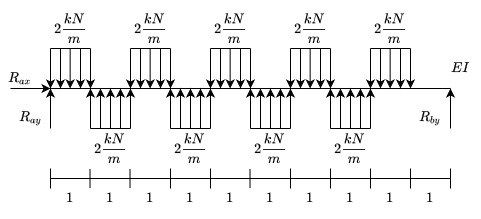
\includegraphics[width=\textwidth]{FBD/FBD_1.jpg}
\caption{Free Body Diagram for Problem 1}
\label{FBD_1}
\end{figure}

\begin{equation}
\begin{split}
	&\uparrow \sum F_y = R_a - 2(1) + 2(1) - 2(1) + 2(1) - 2(1) + 2(1) - 2(1) + 2(1) - 2(1) + R_b = 0 \\
 	&\rightarrow \sum F_x = 0 \\
 	&\circlearrowleft \sum M_A = -2(1)\left(\frac{1}{2}\right) + 2(1)\left(\frac{3}{2}\right) - 2(1)\left(\frac{5}{2}\right) + 2(1)\left(\frac{7}{2}\right) - 2(1)\left(\frac{9}{2}\right) + 2(1)\left(\frac{11}{2}\right) \\ 
	& - 2(1)\left(\frac{13}{2}\right) + 2(1)\left(\frac{15}{2}\right) - 2(1)\left(\frac{17}{2}\right) + R_b(10) = 0 \\
	& \\
	& R_b = \frac{9}{10} \\
	& R_a = \frac{11}{10} \\
\end{split}
\label{problem1_reaction_equation}
\end{equation}

\begin{equation}
\begin{split}
	&\uparrow \sum F_y = R_a - 2(1) + 2(1) - 2(1) + 2(1) - 2(1) + 2(1) - 2(1) + 2(1) - 2(1) + R_b = 0 \\
 	&\rightarrow \sum F_x = 0 \\
 	&\circlearrowleft \sum M_A = -2(1)\left(\frac{1}{2}\right) + 2(1)\left(\frac{3}{2}\right) - 2(1)\left(\frac{5}{2}\right) + 2(1)\left(\frac{7}{2}\right) - 2(1)\left(\frac{9}{2}\right) + 2(1)\left(\frac{11}{2}\right) \\ 
	& - 2(1)\left(\frac{13}{2}\right) + 2(1)\left(\frac{15}{2}\right) - 2(1)\left(\frac{17}{2}\right) + R_b(10) = 0 \\
	& \\
	& R_b = \frac{9}{10} \\
	& R_a = \frac{11}{10} \\
\end{split}
\label{problem1_reaction_solution}
\end{equation}

\begin{equation}
    \begin{split}
    & EI \frac{\delta^2 v}{\delta x^2} = \frac{11}{10}<x-0>^1 - <x-0>^2 +  2<x-1>^2 - 2<x-2>^2 +  2<x-3>^2 \\
    & - 2<x-4>^2  +  2<x-5>^2 - 2<x-6>^2  +  2<x-7>^2 - 2<x-8>^2 +  <x-9>^2  \\
    & EI \frac{\delta v}{\delta x} =  \frac{11}{20}<x-0>^2 - \frac{1}{3}<x-0>^3 +  \frac{2}{3}<x-1>^3 - \frac{2}{3}<x-2>^3 +  \frac{2}{3}<x-3>^3 \\
    & - \frac{2}{3}<x-4>^3  +  \frac{2}{3}<x-5>^3 - \frac{2}{3}<x-6>^3  +  \frac{2}{3}<x-7>^3 - \frac{2}{3}<x-8>^3 +  \frac{1}{3}<x-9>^3  \\
    & EI v(x) = \frac{11}{60}<x-0>^3 - \frac{1}{12}<x-0>^4 +  \frac{1}{6}<x-1>^4 - \frac{1}{6}<x-2>^4 +  \frac{1}{6}<x-3>^4 \\
    & - \frac{1}{6}<x-4>^4  +  \frac{1}{6}<x-5>^4 - \frac{1}{6}<x-6>^4  +  \frac{1}{6}<x-7>^4 - \frac{1}{6}<x-8>^4 +  \frac{1}{12}<x-9>^4  \\
    \end{split}
\label{problem1_equations}
\end{equation}

\subsection{Problem 2}

\begin{figure}[h]
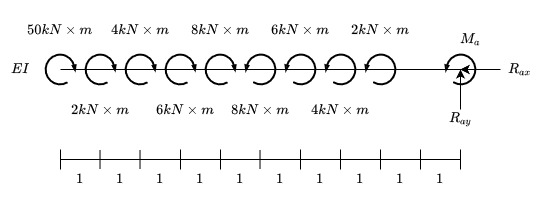
\includegraphics[width=\textwidth]{FBD/FBD_2.jpg}
\caption{Free Body Diagram for Problem 2}
\label{FBD_2}
\end{figure}

\subsection{Problem 3}

\begin{figure}[h]
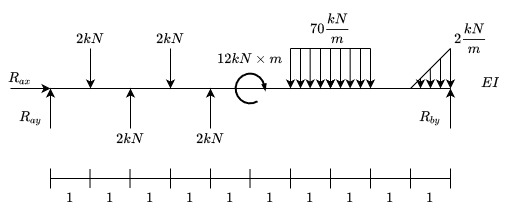
\includegraphics[width=\textwidth]{FBD/FBD_3.jpg}
\caption{Free Body Diagram for Problem 3}
\label{FBD_3}
\end{figure}

\subsection{Problem 4}

\begin{figure}[h]
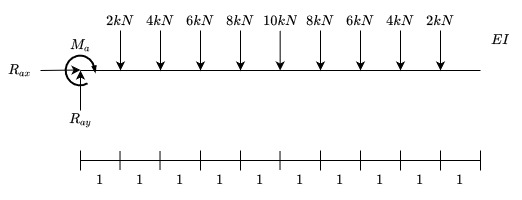
\includegraphics[width=\textwidth]{FBD/FBD_4.jpg}
\caption{Free Body Diagram for Problem 4}
\label{FBD_4}
\end{figure}

\subsection{Problem 5}

\begin{figure}[h]
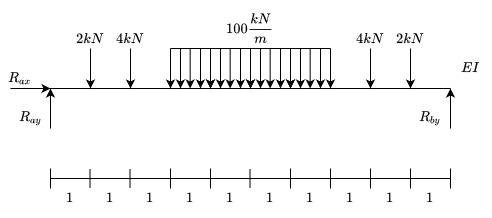
\includegraphics[width=\textwidth]{FBD/FBD_5.jpg}
\caption{Free Body Diagram for Problem 5}
\label{FBD_5}
\end{figure}

\subsection{Problem 6}

\begin{figure}[h]
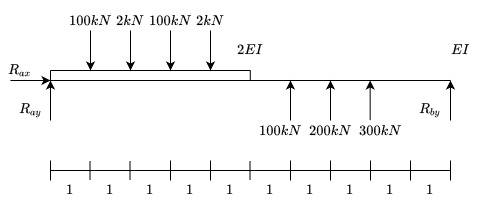
\includegraphics[width=\textwidth]{FBD/FBD_6.jpg}
\caption{Free Body Diagram for Problem 6}
\label{FBD_6}
\end{figure}

\subsection{Problem 7}

\begin{figure}[h]
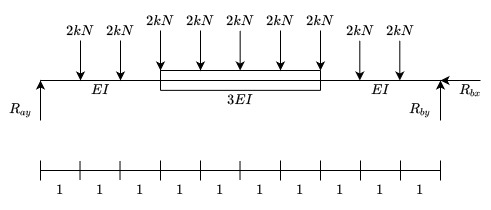
\includegraphics[width=\textwidth]{FBD/FBD_7.jpg}
\caption{Free Body Diagram for Problem 7}
\label{FBD_7}
\end{figure}


\section{Problem Solution} \label{Solutions}
\subsection{Problem 1}
\lipsum[1]
\subsection{Problem 2}
\lipsum[1]
\subsection{Problem 3}
\lipsum[1]
\subsection{Problem 4}
\lipsum[1]
\subsection{Problem 5}
\lipsum[1]
\subsection{Problem 6}
\lipsum[1]
\subsection{Problem 7}
\lipsum[1]

\section{Results and Discussion} \label{Results}
\subsection{Problem 1}
\lipsum[1]
\subsection{Problem 2}
\lipsum[1]
\subsection{Problem 3}
\lipsum[1]
\subsection{Problem 4}
\lipsum[1]
\subsection{Problem 5}
\lipsum[1]
\subsection{Problem 6}
\lipsum[1]
\subsection{Problem 7}
\lipsum[1]

\section{Conclusions} \label{Conclusions}
\lipsum[1]

\section{Appendix}
\lipsum[1]

\bibliographystyle{apalike}
\bibliography{references}

\end{document}
